%! TEX root = main.tex

\graphicspath{{00_Images/02_chapter/}}

\chapter{Theory of Electromechanical Analogies}

The goal of the analogy theory is to represent mechanical and acoustical systems using the formalism of electrical circuit theory. This is not merely a notational convenience: because electrical circuit analysis offers a complete, systematic, and computationally powerful set of tools, Kirchhoff's laws, impedance combinations, Thévenin and Norton equivalents, frequency-domain methods, the ability to map a mechanical or acoustical system onto an equivalent electrical network allows all of these tools to be applied directly to the analysis of transducers, loudspeaker enclosures, and microphone capsules. The approach proceeds domain by domain: the electrical domain is reviewed first, the mechanical domain is introduced next by identifying its power variables and constitutive elements, and the two analogies that connect the two domains are then established and compared.

\section{The Electrical Domain}

The electrical domain is characterized by two power variables: voltage \(v\) (the potential difference between two nodes, measured in volts) and current \(i\) (the flow of charge through a branch, measured in amperes). The instantaneous electrical power delivered to a two-terminal element is \(P_E = v i\). Three ideal passive elements are used to model any linear, time-invariant (LTI) electrical network.

\paragraph{Resistor} A resistor of value \(R\) satisfies Ohm's law:
\[
v = R i
\]
It dissipates power (\(\bar P = R i_{\mathrm{RMS}}^2\)) and introduces no phase shift between voltage and current.

\paragraph{Capacitor} A capacitor of capacitance \(C\) (measured in farads, \(\si{\farad}\)) stores energy in its electric field. The constitutive relation is:
\[
i = C \frac{dv}{dt}
\qquad\Leftrightarrow\qquad
v(t) = \frac{1}{C}\int_0^t i(\tau) d\tau
\qquad\xrightarrow{\ \mathcal{L}\ }\qquad
V(s) = \frac{1}{sC} I(s)
\]
In steady sinusoidal operation the impedance is \(Z_C = 1/(j\omega C)\): the current leads the voltage by \(\pi/2\), and no net power is dissipated over one period.

\paragraph{Inductor} An inductor of inductance \(L\) (measured in henrys, \(\si{\henry}\)) stores energy in its magnetic field. The constitutive relation is:
\[
v = L \frac{di}{dt}
\qquad\Leftrightarrow\qquad
i(t) = \frac{1}{L}\int_0^t v(\tau) d\tau
\qquad\xrightarrow{\ \mathcal{L}\ }\qquad
I(s) = \frac{1}{sL} V(s)
\]
In sinusoidal operation the impedance is \(Z_L = j\omega L\): the voltage leads the current by \(\pi/2\), and no net power is dissipated.

\begin{figure}[!htb]
    \centering
    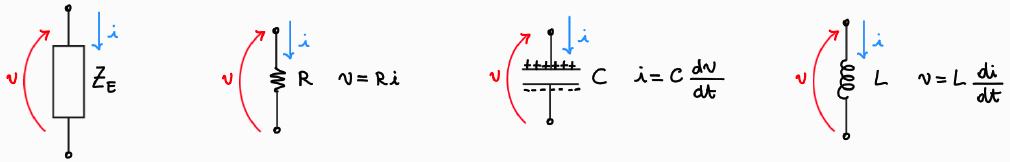
\includegraphics[width=0.85\textwidth]{electrical_elements.png}
    \caption{The three passive elements of the electrical domain: resistor (left), capacitor (center), and inductor (right), with their constitutive relations in the time domain}
\end{figure}

\paragraph{Alessandro Volta and the invention of the capacitor} A brief historical note is warranted here. Alessandro Volta (Como, 1745-1827), Professor of Physics at the University of Pavia from 1778, is universally known as the inventor of the electrochemical battery (the voltaic pile, demonstrated in 1799 and presented to Napoleon in Paris in 1801). Less commonly noted is that Volta had conceived and built the electrical condenser, the capacitor, even earlier, in 1789, as part of his work on electrometers for measuring electrostatic charge. Volta is therefore the inventor of not one but two of the three fundamental passive circuit elements, the capacitor and, indirectly through the battery, the voltage source. The unit of potential difference, the volt, commemorates his contributions, and the first international congress of physics held at Como in 1927, on the centenary of his death, brought together an extraordinary assembly of Nobel laureates including Lorentz, Planck, Bohr, Heisenberg, Fermi, and Pauli.

\section{The Mechanical Domain}

The mechanical domain is characterized by two power variables that play roles analogous to voltage and current in the electrical domain. The relevant variables for a one-dimensional mechanical system (such as the axial motion of a loudspeaker diaphragm) are force \(F\) (measured in newtons, \(\si{\newton}\)) and velocity \(u\) (measured in metres per second, \(\si{\meter\per\second}\)). The instantaneous mechanical power transmitted through a one-port mechanical element is:
\[
P_M = F u
\]
This is directly analogous to \(P_E = v i\) in the electrical domain, and it is this power equivalence that forms the physical basis for all electromechanical analogies. The displacement of the element is related to its velocity by \(x = \int u dt\). Three ideal mechanical elements, mass, spring (characterized by its compliance), and damper, describe the inertial, elastic, and dissipative behavior of any linear mechanical system.

\begin{figure}[!htb]
    \centering
    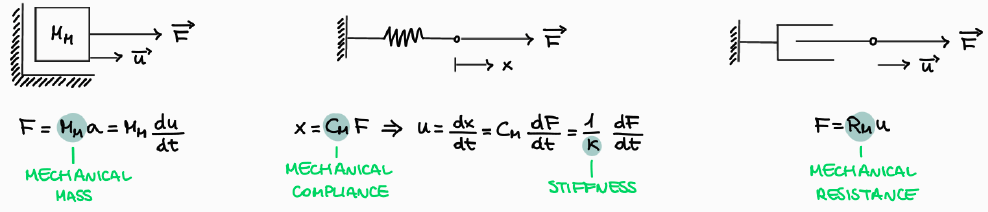
\includegraphics[width=0.80\textwidth]{mechanical_blocks.png}
    \caption{The three fundamental mechanical elements. Mass (left): \(F = M_M du/dt\). Spring with compliance \(C_M\) (center): \(u = C_M dF/dt\). Viscous damper (right): \(F = R_M u\). Each element is characterized by its constitutive relation between force and velocity}
\end{figure}

\subsection{Mechanical Mass}

The mechanical mass \(M_M\) (in kilograms, \(\si{\kilo\gram}\)) represents the inertia of a rigid body. By Newton's second law, the net force required to accelerate the mass is:
\[
F = M_M \frac{du}{dt}
\qquad\Leftrightarrow\qquad
u(t) = \frac{1}{M_M}\int_0^t F(\tau) d\tau
\]
In sinusoidal operation, with \(u = \tilde{u} e^{j\omega t}\), the force is \(F = j\omega M_M u\); the mechanical impedance of the mass is therefore \(Z_{M,\text{mass}} = j\omega M_M\), which increases linearly with frequency. The mass stores kinetic energy \(\frac{1}{2}M_M u^2\) but dissipates none; it is the mechanical analogue of the electrical inductor, because both elements oppose changes in the flow variable (current or velocity) by relating that variable to the time integral of the driving variable (voltage or force).

\subsection{Mechanical Compliance (Spring)}

The mechanical compliance \(C_M\) (in meters per newton, \(\si{\meter\per\newton}\)) is the reciprocal of the mechanical stiffness \(K = 1/C_M\). Hooke's law states that the displacement of a spring under a force \(F\) is proportional to the force:
\[
x = C_M F
\]
Differentiating both sides with respect to time gives the velocity-force constitutive relation:
\[
u = \frac{dx}{dt} = C_M \frac{dF}{dt}
\qquad\Leftrightarrow\qquad
F(t) = \frac{1}{C_M}\int_0^t u(\tau) d\tau
\]
In sinusoidal operation the mechanical impedance of the spring is \(Z_{M,\text{spring}} = 1/(j\omega C_M)\), which decreases with frequency and dominates the response at low frequencies. The spring stores potential energy \(\frac{1}{2}K x^2 = x^2/(2C_M)\) but dissipates none; it is the mechanical analogue of the electrical capacitor, because both elements relate the flow variable to the time integral of the driving variable (charge \(= \int i dt\) for the capacitor; displacement \(= \int u dt\) for the spring). The compliance \(C_M\) is thus the mechanical quantity that corresponds most naturally to electrical capacitance, and it is the parameter used to characterize the suspension of a loudspeaker or the diaphragm of a microphone.

\subsection{Mechanical Resistance (Damper)}
\label{ssc:523}

The mechanical damper (or dashpot) \(R_M\) (in newton-seconds per meter, \(\si{\newton\second\per\meter}\)) models viscous friction losses, the resistive force opposing velocity that arises from air friction, internal material damping in the suspension, or deliberate damping materials. Its constitutive relation is:
\[
F = R_M u
\qquad\Leftrightarrow\qquad
u = \frac{F}{R_M}
\]
The mechanical impedance of the damper is \(Z_{M,\text{damper}} = R_M\), independent of frequency. Power is dissipated as heat at the rate \(\bar P = R_M u_{\mathrm{RMS}}^2\). The damper is the mechanical analogue of the electrical resistor. Note that its reciprocal \(G_M = 1/R_M\) is the mechanical conductance (or mobility), measured in meters per newton-second; this quantity will arise naturally in the admittance analogy.

\paragraph{D'Alembert's principle for the diaphragm} In the loudspeaker, the voice coil exerts the driving force \(F_C = Bl i\) on the diaphragm, which is simultaneously subject to the spring restoring force of the suspension (\(F_S = x/C_{MS}\)), the viscous damping force (\(F_D = R_{MS} u\)), and its own inertial force (\(F_M = M_{MD} du/dt\)). D'Alembert's principle requires these forces to balance at every instant:
\[
F_C = F_S + F_D + F_M
= \frac{1}{C_{MS}}\int_0^t u(\tau) d\tau + R_{MS} u + M_{MD} \frac{du}{dt}
\]
This single equation, the mechanical equation of motion of the loudspeaker diaphragm, is the mechanical counterpart of Kirchhoff's voltage law for a series RLC circuit, a connection that the impedance analogy will make precise.

\section{Impedance and Admittance Analogies}

The objective of the analogy theory is to establish a one-to-one correspondence 
between the variables and elements of the mechanical domain and those of the 
electrical domain, so that an equivalent electrical circuit can be drawn for any 
mechanical system and analyzed by standard network methods. Two distinct analogies 
exist, each resting on a different identification of the mechanical power variables 
with the electrical ones. Both are physically valid; the choice between them is 
governed by considerations of topological clarity and computational convenience.

\subsection{Impedance Analogy (Type I)}

The variable mapping is:
\[
F \;\leftrightarrow\; v, \qquad u \;\leftrightarrow\; i
\]
so that the mechanical impedance \(Z_M = F/u\) maps directly onto the electrical 
impedance \(Z_E = v/i\).

\paragraph{Mechanical Mass}
\[
F = M_M \frac{du}{dt}
\;\xrightarrow{F\to v,\;u\to i}\;
v = M_M \frac{di}{dt} = L \frac{di}{dt}
\qquad\Longrightarrow\qquad
L = M_M
\]
The mechanical mass corresponds to an inductor.

\paragraph{Mechanical Compliance}
\[
u = C_M \frac{dF}{dt}
\;\xrightarrow{u\to i,\;F\to v}\;
i = C_M \frac{dv}{dt} = C \frac{dv}{dt}
\qquad\Longrightarrow\qquad
C = C_M
\]
The mechanical compliance corresponds to a capacitor.

\paragraph{Mechanical Resistance (Damper)}
\[
F = R_M u
\;\xrightarrow{F\to v,\;u\to i}\;
v = R_M i
\qquad\Longrightarrow\qquad
R = R_M
\]
The mechanical damper corresponds to a resistor.

\paragraph{Summary and topological rule}
\[
M_M \;\leftrightarrow\; L, \qquad C_M \;\leftrightarrow\; C, 
\qquad R_M \;\leftrightarrow\; R
\]
Since velocity maps to current, mechanical elements that share the same velocity 
experience the same current in the electrical circuit; they are therefore connected 
in series.

\subsection{Admittance Analogy (Type II)}

The variable mapping is:
\[
F \;\leftrightarrow\; i, \qquad u \;\leftrightarrow\; v
\]
so that the mechanical admittance \(Y_M = u/F\) maps directly onto the electrical 
admittance \(Y_E = i/v\).

\paragraph{Mechanical Mass}
\[
F = M_M \frac{du}{dt}
\;\xrightarrow{F\to i,\;u\to v}\;
i = M_M \frac{dv}{dt} = C \frac{dv}{dt}
\qquad\Longrightarrow\qquad
C = M_M
\]
The mechanical mass corresponds to a capacitor.

\paragraph{Mechanical Compliance}
\[
u = C_M \frac{dF}{dt}
\;\xrightarrow{u\to v,\;F\to i}\;
v = C_M \frac{di}{dt} = L \frac{di}{dt}
\qquad\Longrightarrow\qquad
L = C_M
\]
The mechanical compliance corresponds to an inductor.

\paragraph{Mechanical Resistance (Damper)}
\[
F = R_M u
\;\xrightarrow{F\to i,\;u\to v}\;
i = R_M v
\qquad\Longrightarrow\qquad
G_E = R_M, \quad R_E = \frac{1}{R_M}
\]
The mechanical damper corresponds to a conductance \(G_E = R_M\), represented 
in circuit diagrams as a resistor of value \(R_E = 1/R_M\).

\paragraph{Summary and topological rule}
\[
M_M \;\leftrightarrow\; C, \qquad C_M \;\leftrightarrow\; L, 
\qquad R_M \;\leftrightarrow\; G_E
\]
Since velocity maps to voltage, mechanical elements that share the same velocity 
experience the same voltage in the electrical circuit; they are therefore connected 
in parallel. This preserves the physical topology of the mechanical system: 
just as mass, compliance, and damper all connect the moving diaphragm to the fixed 
basket, the corresponding electrical elements all connect the same two nodes in the 
parallel circuit.

\begin{figure}[!htb]
    \centering
    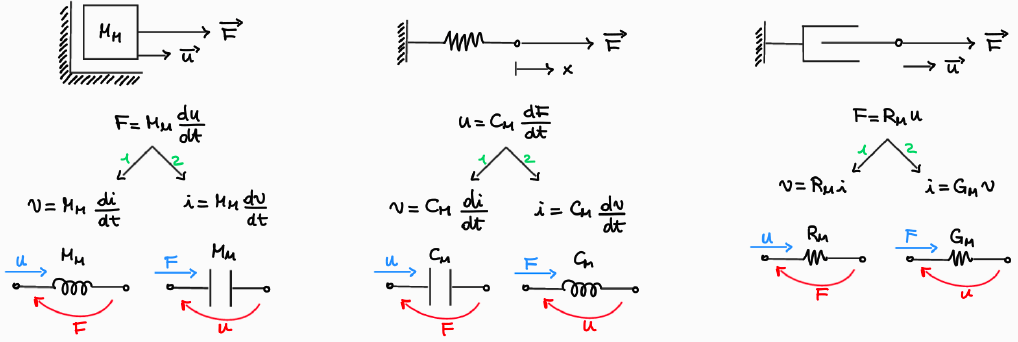
\includegraphics[width=0.85\textwidth]{impedance_admittance_analogies.png}
    \caption{Comparison of the impedance analogy (left) and the admittance analogy 
    (right) for the three fundamental mechanical elements. Under the impedance analogy, 
    common-velocity elements are in series; under the admittance analogy, they are in 
    parallel, preserving the visual topology of the mechanical system}
    \label{fig:analogiesComparison}
\end{figure}

\subsection{Summary of the Two Analogies}
\label{ssc:533}

Both analogies are mathematically equivalent: they produce identical predictions for all physical observables (impedance magnitude, frequency response, power, etc.) once the correct network topology is adopted. The choice is therefore one of convention and convenience. In loudspeaker analysis, where the diaphragm–suspension assembly has a natural parallel topology (all elements share the same velocity relative to the fixed basket), the admittance analogy is most common. In microphone and transmission-line analysis, where elements are naturally in series (they carry the same current or force in sequence), the impedance analogy may be preferred. The two choices will be kept explicit throughout this text, and the relevant analogy will be stated whenever a new equivalent circuit is introduced.

\begin{table}[!htb]
\centering
\renewcommand{\arraystretch}{1.3}
\begin{tabular}{|c|c|c|}
\hline
\textbf{Mechanical element} & \textbf{Impedance analogy} & \textbf{Admittance analogy} \\
& \textbf{Type I} & \textbf{Type II} \\
\hline
Force \(F\) & Voltage \(v\) & Current \(i\) \\
Velocity \(u\) & Current \(i\) & Voltage \(v\) \\
\hline
Mass \(M_M\) & Inductor \(L = M_M\) & Capacitor \(C = M_M\) \\
Compliance \(C_M\) & Capacitor \(C = C_M\) & Inductor \(L = C_M\) \\
Damper \(R_M\) & Resistor \(R = R_M\) & Conductance \(G = 1/R_M\) \\
\hline
Common-velocity elements & Series circuit & Parallel circuit \\
\hline
\end{tabular}
\caption{Variable mappings and element correspondences for the impedance analogy (Type I) and the admittance analogy (Type II). Both analogies are physically equivalent and produce the same predictions when the full network is analyzed}
\end{table}

\paragraph{Mechanical impedance and power} Regardless of which analogy is chosen, the mechanical impedance of a one-port element is defined as:
\[
Z_M = \frac{F}{u} = R_M + j X_M
\]
where \(R_M\) is the resistive (power-dissipating) part and \(X_M = \omega M_M - 1/(\omega C_M)\) is the reactive (energy-storing) part. The mean mechanical power delivered to the element is:
\[
\bar P_M = R_M u_{\mathrm{RMS}}^2
\]
confirming that only the resistive part of the mechanical impedance contributes to long-term energy dissipation, in complete analogy with the electrical case \(\bar P_E = \mathcal{R}\{Z_E\} I_{\mathrm{RMS}}^2\). This result will be used extensively in the analysis of loudspeaker efficiency and power handling in the chapters that follow.